% =====================================================================
%  Chapitre 4 -- Entrainement, applications, projet
%  Partie b : fuite temporelle, projet, synthese du module
% =====================================================================

\begin{frame}{Le piège qui ruine une évaluation : la fuite temporelle}
\begin{center}
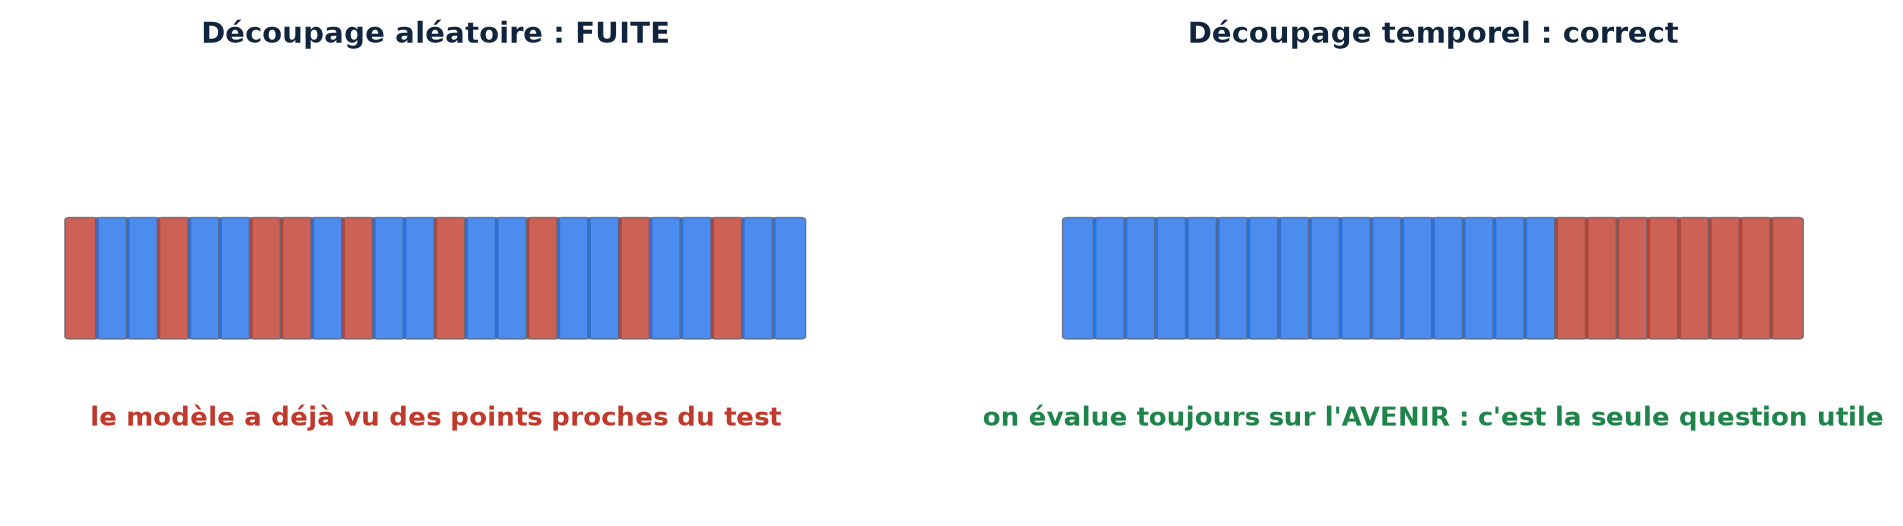
\includegraphics[width=0.92\textwidth]{u07_fuite.png}
\end{center}
\vspace{1mm}
\begin{wbox}[L'erreur la plus fréquente du domaine]
Découper une série temporelle \textbf{au hasard} place des points futurs dans
l'entraînement : le score est flatteur et ne signifie rien.

Pour une séquence, le découpage est \textbf{temporel} --- toujours.
\end{wbox}
\end{frame}

\begin{frame}{Les métriques, selon la tâche}
\begin{columns}[t]
\begin{column}{0.32\textwidth}
\begin{ebox}[Classification]
Exactitude, précision, rappel, F1 --- comme au module CNN. Attention aux
classes déséquilibrées.
\end{ebox}
\end{column}
\begin{column}{0.32\textwidth}
\begin{ebox}[Prévision]
RMSE, MAE, et surtout une comparaison avec une \textbf{référence naïve}.
\end{ebox}
\end{column}
\begin{column}{0.32\textwidth}
\begin{ebox}[Génération]
Perplexité, et une lecture humaine des échantillons --- les métriques
automatiques ne suffisent pas.
\end{ebox}
\end{column}
\end{columns}
\vspace{2mm}
\begin{kbox}[La question à se poser avant toute métrique]
« Mon jeu de test est-il \emph{dans l'avenir} de mon jeu d'entraînement ? »
\end{kbox}
\end{frame}

\begin{frame}{Le projet du module, de bout en bout}
\begin{center}
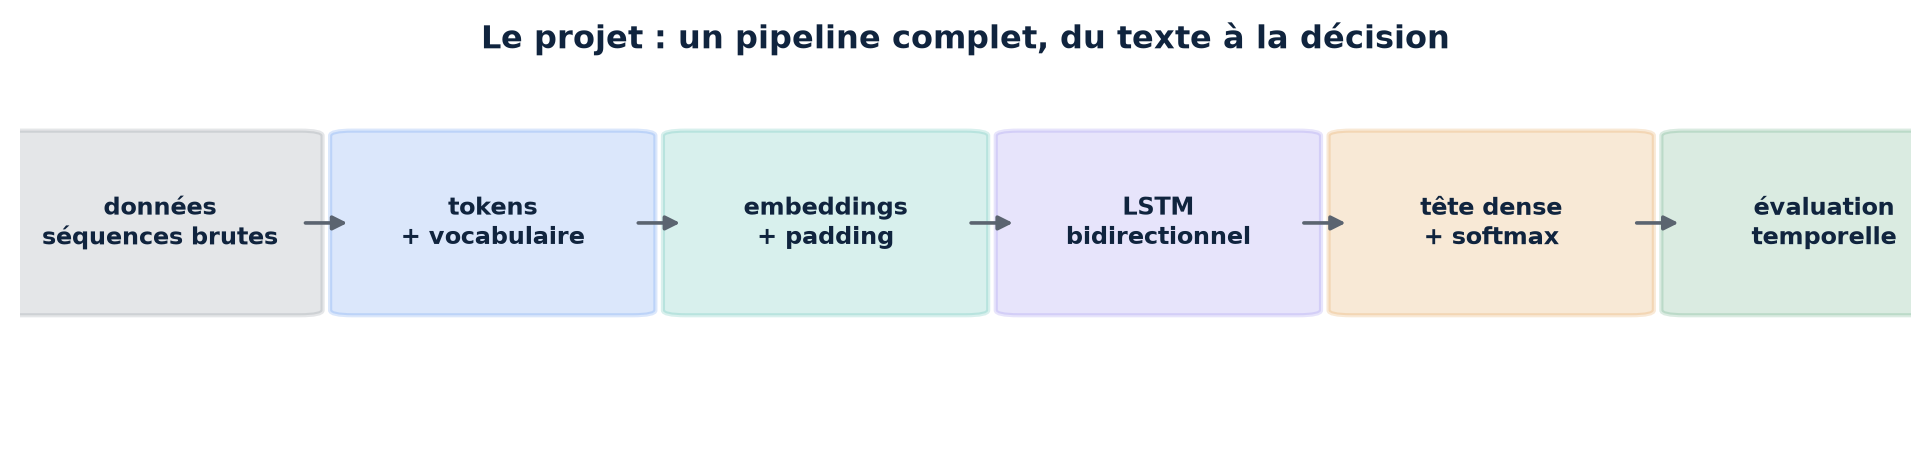
\includegraphics[width=0.96\textwidth]{u08_projet.png}
\end{center}
\vspace{1mm}
\begin{itemize}
  \item Deux sujets au choix : \textbf{classifier des critiques} ou
  \textbf{prédire une trajectoire}.
  \item Le notebook du projet fournit le squelette et le barème ; vous
  remplissez les zones « À vous ».
\end{itemize}
\end{frame}

\begin{frame}{Barème du projet (20 points)}
\begin{center}
\small
\begin{tabular}{@{}p{0.62\textwidth}r@{}}
\toprule
\textbf{Critère} & \textbf{Points} \\
\midrule
Le notebook s'exécute de bout en bout sans erreur & 4 \\
Protocole temporel correct (pas de fuite, découpage justifié) & 4 \\
Résultat mesuré et comparé à une référence naïve & 4 \\
Une expérience contrôlée (RNN vs LSTM vs bidirectionnel) & 4 \\
Analyse des erreurs : où le modèle se trompe, et pourquoi & 2 \\
Conclusion critique : trois limites honnêtes & 2 \\
\bottomrule
\end{tabular}
\end{center}
\vspace{1mm}
\begin{wbox}[Rappel de la règle du cours]
Un chiffre annoncé sans la commande qui l'a produit ne vaut rien.
Toute valeur du rapport doit être reproductible (graine fixée).
\end{wbox}
\end{frame}

\begin{frame}{Quiz 6 --- projet et évaluation}
\begin{qbox}[Question 1]
Pour évaluer un modèle de prévision de trafic, on découpe le jeu :
\begin{itemize}
  \item[(a)] au hasard, 80/20 \quad (b) dans l'ordre du temps
  \quad (c) au hasard, avec stratification
\end{itemize}
\end{qbox}
\begin{qbox}[Question 2]
Avant de célébrer un LSTM, on compare à :
\begin{itemize}
  \item[(a)] un Transformer \quad (b) une référence naïve (dernière valeur)
  \quad (c) rien, la métrique suffit
\end{itemize}
\end{qbox}
\begin{qbox}[Question 3]
Un score de 95 % obtenu par découpage aléatoire sur une série temporelle :
\begin{itemize}
  \item[(a)] est excellent \quad (b) doit être repris avec un découpage temporel
  \quad (c) prouve la qualité du modèle
\end{itemize}
\end{qbox}
\begin{solbox}[Réponses]
\textbf{1.} (b). \quad \textbf{2.} (b) : sans référence, aucun chiffre n'est
interprétable. \quad \textbf{3.} (b) : c'est presque certainement une fuite.
\end{solbox}
\end{frame}

\begin{frame}{Synthèse du module}
\begin{kbox}[Les six réflexes à emporter]
\begin{enumerate}
  \item Une séquence est \textbf{ordonnée} et de longueur libre : ni aplatissement,
  ni fenêtre.
  \item La même cellule déroulée : $h_t = \tanh(W_x x_t + W_h h_{t-1} + b)$.
  \item Le gradient le long du temps est un produit : il s'évanouit ou explose.
  \item Le LSTM le répare par un \textbf{convoyeur} : $C_t = f_t \odot C_{t-1}
  + i_t \odot \tilde{C}_t$ ; la GRU en est la version allégée.
  \item Teacher forcing à l'entraînement, inférence libre à l'évaluation :
  ce sont deux régimes.
  \item Le protocole temporel prime sur le modèle : sans lui, tout score est
  suspect.
\end{enumerate}
\end{kbox}
\end{frame}

\begin{frame}{Et après ?}
\begin{columns}[t]
\begin{column}{0.48\textwidth}
\begin{ebox}[Ce que ces bases ouvrent]
\begin{itemize}
  \item Les \textbf{Transformers}, qui généralisent l'attention et suppriment
  la récurrence.
  \item Les modèles de langue (GPT, BERT) : attention + très grandes données.
  \item L'alignement de séquences en biologie, la parole, la traduction.
\end{itemize}
\end{ebox}
\end{column}
\begin{column}{0.48\textwidth}
\begin{ebox}[Les TP et le projet]
\begin{itemize}
  \item TP1 : embeddings et séquences.
  \item TP2 : RNN sur série temporelle.
  \item TP3 : LSTM/GRU sur les critiques.
  \item Projet : votre pipeline de bout en bout.
\end{itemize}
\end{ebox}
\end{column}
\end{columns}
\vspace{1.5mm}
\begin{solbox}[Fin du module]
Les notebooks sont livrés exécutés ; rejouez-les, modifiez-les, mesurez.
C'est en écrivant les gradients à la main qu'on comprend ce que fait le
machine à notre place.
\end{solbox}
\end{frame}
